\section{Web-Game [R]}
\setauthor{Rafetseder Tobias}
\subsection{Frontend [R]}
Für die Umsetzung des Frontends wird p5.js beziehungsweise p5.play.js verwendet. 
Eine detaillierte Beschreibung zu diesem JavaScript-Bibliothek und wie man es in ein Projekt einbinden kann, wird in Kapitel \ref{subsection:p5js} genau beschrieben.
p5.play.js basiert auf einer Sprite Klasse. Diese Sprite-Klasse hat einige praktische vordefinierte Funktionen für Collisiondetection oder Animation Support. 
Um einen Sprite zu erstellen, wird einfach die Funktion createSprite() aufgerufen.
\\
\begin{lstlisting}[language=Java,label=lst:impl:createSprite]
    function setup() {
        createCanvas(1920,1080);
        // create a sprite
        createSprite(50,50,30,30);
    }

    function draw() {
        // draw all the sprites added to the sketch so far
        // the positions will be updated automatically at every cycle
        drawSprites();
    }
\end{lstlisting}


Es ist zu beachten, dass die ersten 2 Parameter der Funktion jeweils die Position am Bildschirm in Pixel angeben, und die letzten 2 die Breite und die Höhe definieren.
Das Ergebnis:
\begin{figure}[H]
    \centering
    
\includegraphics[scale=1]{pics/simpleSprite.PNG}
    \caption{Einfacher Sprite}
\end{figure}

Es ist noch nicht viel zu sehen, nur ein simpler Sprite, der default-mäßig ein einfaches Rechteck mit zufälliger Farbe auf einer Position erschienen ist.
Für den Player, den man in dem Web-Game sieht, wird diese Sprite-Klasse noch um ein paar Attribute erweitert:

\begin{figure}[H]
    \centering
    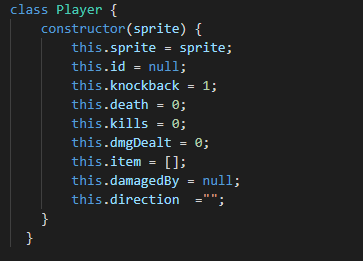
\includegraphics[scale=1]{pics/playerClass.PNG}
    \caption{Player-Klasse}
\end{figure}

Zum Erstellen der Player-Klasse wird zwar ein Sprite benötigt, damit der Player am Bildschirm angezeigt wird, aber Attribute wie:
\begin{compactitem}
    \item id: Zur eindeutigen Identifizierung
    \item knockback: Wert, der erhöht wird, desto öfter man getroffen wird; desto höher der Wert, desto weiter wird man von Projektilen weggestoßen
    \item death: Anzahl, wie oft man gestorben ist
    \item kills: Anzahl an Kills, die man gemacht hat
    \item dmgDealt: Anzahl, wie oft man jemanden getroffen hat
    \item item: Array von Items, die man gerade besitzt
    \item direction: String, der die Richtung angibt, in die man gerade schaut (links oder rechts)
\end{compactitem}

Während des Spiels werden auf der Map Items gespawned. Welcher Algorithmus dahinter steckt, wird im Kapitel TODO genauer beschrieben.
Es wird zwischen 5 unterschiedlichen Items entschieden. Eine Item-Klasse hat ähnlich wie die Player-Klasse als Hauptbestandteil einen Sprite, doch auch hier werden noch weitere Attribute benötigt.

\begin{figure}[H]
    \centering
    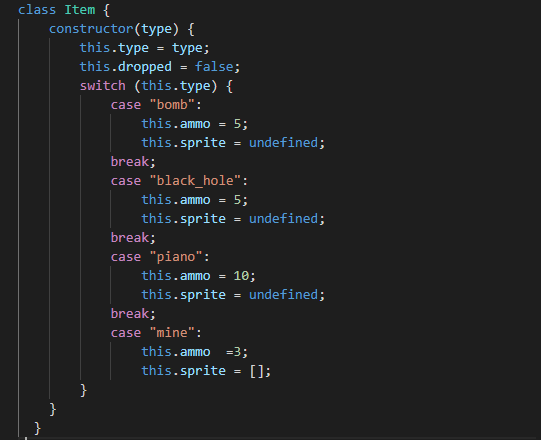
\includegraphics[scale=1]{pics/itemClass.PNG}
    \caption{Item-Klasse}
\end{figure}

\begin{compactitem}
    \item type: Gibt den Typ des Items andere
    \item dropped: Gibt an, ob das Item irgendwo auf der Umgebung gelandet ist
    \item ammo: Anzahl, wie oft man das Item benutzen kann
\end{compactitem}

Je nachdem, welchen Typ das Item bekommen hat, wird auch die Anzahl wie oft
 man es benutzen kann, verändert. 
Wurde es zum Beispiel zum Type "bomb", kann man 5 Mal eine Bombe werfen.
\\
Bei dem Typ "mine", also einer Mine, kann man mehrere Minen gleichzeitig legen, deshalb ist das Sprite-Attribut auch ein Array.
Bei den anderen Items kann immer nur ein Sprite davon existieren.

\subsubsection{Die Items}
Grundsätzlich gibt es 5 unterschiedliche Items in Scribble-Fight. Je nachdem, welches Item man aufgesammelt hat, kann man verschiedene Fähigkeiten aktivieren.
Für jedes Item existiert eine physics-Methode, die in der Draw-Funktion aufgerufen wird. 

\textbf{Keyboard-Access}
\\
Durch p5.js kann man sehr leicht auf die Tastatur zugreifen. Mithilfe von ASCII Code greift man auf die einzelnen Tasten zu.
Mit der p5.js Methode <keyWentDown(Key)> wird überprüft, ob die Taste gerade gedrückt wurde.

\begin{lstlisting}[caption=Keyboard-Access,language=Java,label=lst:impl:keyboard-access]
    // E
    if (keyWentDown(69)) {
        bombAttack();
    }
    // Q
    if (keyWentDown(81)) {
        blackHoleAttack();
    }
    // R
    if (keyWentDown(82)) {
        pianoTime();
    }
    // C
    if (keyWentDown(67)) {
        placeMine();
    }
    // F
    if (keyWentDown(70)) {
        makeMeSmall();
    }
\end{lstlisting}

\textbf{Bomb}
\\
\textit{Das Bombem-Item wird mit der Taste <E> aktiviert.}
\\
Durch p5.play.js kann man mit <sprite.velocity.y> die vertikale Geschwindigkeit eines Sprites verändern. Dadurch kann eine Gravitation simuliert werden.
Außerdem kann man mit <sprite.bounce(otherSprite)> Sprites an anderen Sprites oder Gruppen von Sprites 'abspringen' lassen. Dies wird benutzt, damit die Bombe an der Umgebung abprallt
Danach wird mit <sprite.overlap(myPlayer.sprite)> überprüft, ob eine Bombe mit meinem Spieler-Sprite kollidiert.
Falls ja, wird die Bombe mit <sprite.remove()> entfernt.
Falls nein, wird noch überprüft, ob sich die Bombe außerhalb des Bildschirms befindet, und falls dies zutrifft, wird auch in dem Fall die Bombe entfernt.
\\

\begin{lstlisting}[caption=Bomb Item Physics,language=Java,label=lst:impl:bombGravity]
    // verringern der vertikalen Geschwindigkeit 
    bomb.velocity.y -= GRAVITY;
    // bombe prallt an der Umgebung ab
    bomb.bounce(environment);

    // kollidert die Bombe mit meinem Player
    if(bomb.overlapSprite(myPlayer.sprite)) {
        // my Player gets knocked back
        myPlayer.sprite.getsThrownAway();
        // bomb gets deleted
        bomb.remove();
    } else if(bombIsOutsideMonitor()) {
        // bomb gets deleted
        bomb.remove();
    }

\end{lstlisting}

\textbf{Black Hole}
\\
\textit{Das Black-Hole-Item wird mit der Taste <Q> aktiviert}.
\\
Wie bei dem Bomben-Item wird auch bei dem Black-Hole-Item Gravitation simuliert. Jedoch nur für eine kurze Zeit, bis das Item in der Luft stehen bleibt und in einem Radius alle Spieler, die sich in diesem Radius befinden, anzieht, und diese auch alle Fähigkeiten nimmt.
Um zu überprüfen, wie lange das Item schon existiert, stellt p5.play.js das <life>-Attribut zur Verfügung. Dieser Wert ist ein Countdown, der sich bei jedem Draw-Zyklus um 1 verringert, bis sich das Item dann bei dem Wert 0 selbst löscht.
Ein weiterer wichtiger Punkt ist bei dem Item, wie es Sprites anziehen kann. Dazu wurde die attraction Funktion von p5.play.js (mit leichten Veränderungen) benutzt:

\begin{lstlisting}[caption=Attraction,language=Java,label=lst:impl:attraction]
    // attraction
    if (myPlayer.sprite.overlap(b)) {
        noGravity = true;
        var angle = atan2(myPlayer.sprite.position.y - b.position.y, myPlayer.sprite.position.x - b.position.x);
        if (myPlayer.sprite.velocity.y >= -pixelWidth && myPlayer.sprite.velocity.y <= pixelWidth) {
          myPlayer.sprite.velocity.x -= cos(angle);
        }
        myPlayer.sprite.velocity.y -= sin(angle);
      }

\end{lstlisting}

Die Black-Hole-Physics Funktion sieht also (vereinfacht) so aus:
\\
\begin{lstlisting}[caption=Black Hole Item Physics,language=Java,label=lst:impl:bombGravity]
    // if the item has reached a certain life, make it static and attract players
    if (b.life <= 400) {
        attraction(b);
        b.velocity.y = 0;
        b.velocity.x = 0;
      }

      // if the item has not reached a certain life, let it bounce off the environment
      if (b.life > 400) {
        b.velocity.y -= GRAVITY;
        b.bounce(environment);
      }

      // if the item is outside of the monitor, delete it
      if (b.position.x > windowWidth || b.position.y > windowHeight || b.life == 0) {
        b.remove();
      }

\end{lstlisting}

\textbf{Piano}
\\
\textit{Das Piano-Item wird mit der Taste <R> aktiviert.}



\subsection{Backend [R]}
\subsubsection{Node.js [R]}
\subsubsection{SocketIO [R]}
\subsection{Gamephysics [R]}
\subsection{Hitregistration [R]}
\subsection{Collisiondetection [R]}
\subsection{Regeln und Spielablauf [R]}
\section{Deployment [R]}
\setauthor{Rafetseder Tobias}
\subsection{Docker [R]}
\subsection{Leo-Cloud [R]}

% Ben dein teil kommt hier herein


\section{Map-Erkennung [H]}
\setauthor{Himmetsberger Jonas}
\subsection{Objekterkennung [H]}
\subsubsection{Beschreibung der Funktionalität [H]}
\subsection{Open-CV2 [H]}
\subsubsection{Bildverarbeitungsalgorithmen}
\subsubsection{Umwandlung der Bilder in für das Spiel brauchbare Daten [H]}
\subsection{Kommunikation mit der Lobby via Flask und Flask SocketIO [H]}

\section{KI [H]}
Der erste Punkt ist die Künstliche Intelligenz.
Im Laufe der Ausarbeitung der Diplomarbeit und der damit zusammenhängenden Forschung änderte sich oft die
Vorstellung darüber, wie das Endprodukt (KI) auszusehen hat, beziehungsweise, wie dieses aussehen kann.
Limitierungen, welche vor der Forschung noch nicht bekannt und bewusst waren, begrenzten die Lernfähigkeit der KI.
Auf Probleme, Lösungen und Ergebnisse wird jedoch noch näher in ... eingegangen.
\subsection{Lernen mit OpenAI-Gym [H]}
\subsection{Künstliche Intelligenz Definition [H]}
\subsection{Reinforcement Learning [H]}
\subsection{Die ScribbleFight-KI [H]}
\subsubsection{Beschreibung der Funktionalität [H]}
\subsubsection{Warum Python? [H]}
\subsection{Tensorflow und Keras [H]}
\subsubsection{Tensorflow [H]}
\subsubsection{Keras [H]}



% Siehe tolle Daten in Tab. \ref{tab:impl:data}.

% \begin{table}
%     \centering
%     \begin{tabular}{|lcc|}
%         \hline
%                   & \textbf{Regular Customers} & \textbf{Random Customers} \\ \hline
%         Age       & 20-40                      & \textgreater{}60          \\ \hline
%         Education & university                 & high school               \\ \hline
%     \end{tabular}
%     \caption{Ein paar tabellarische Daten}
%     \label{tab:impl:data}
% \end{table}

% \begin{figure}
%     \centering
%     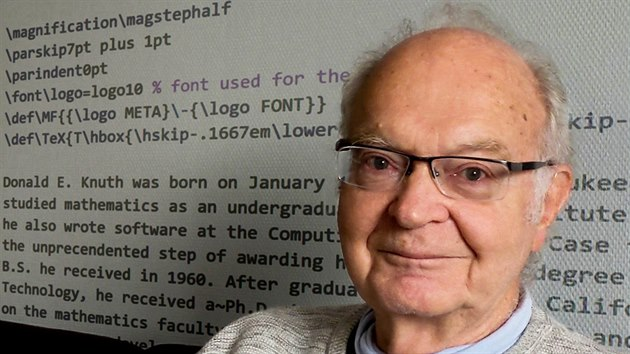
\includegraphics[scale=0.5]{pics/knuthi.jpg}
%     \caption{Don Knuth -- CS Allfather}
%     \label{fig:impl:knuth}
% \end{figure}

% Siehe und staune in Abb. \ref{fig:impl:knuth}.
% \lipsum[6-9]
% Dann betrachte den Code in Listing \ref{lst:impl:foo}.

% \begin{lstlisting}[language=Python,caption=Some code,label=lst:impl:foo]
% # Program to find the sum of all numbers stored in a list (the not-Pythonic-way)

% # List of numbers
% numbers = [6, 5, 3, 8, 4, 2, 5, 4, 11]

% # variable to store the sum
% sum = 0

% # iterate over the list
% for val in numbers:
%     sum = sum+val

% print("The sum is", sum)
% \end{lstlisting}